\input{../MISC/preambule_sacado.tex}
\input{../MISC/environnements_sacado.tex}
\input{../MISC/macro_sacado.tex}
\usepackage{tkz-tab}

\title{Mathématiques 2nde  : le livre sacado}
\author{L'équipe SACADO}

\begin{document}

%\maketitle

\chapter{Titre du chapitre}{Numéro du chapitre}
{URL du parcours}
{
% \begin{CpsCol}
%	\textbf{Les savoir-faire du parcours}
% 	\begin{itemize}
% 		\item SF1
% 		\item SF2
% 	\end{itemize}
% \end{CpsCol}
%
%\begin{His}
%	% Un paragraphe parlant de la vie d'un ou une mathématicien ou mathématicienne
%\end{His}

\begin{ExoDec}{Compétence.}{1234}{1}{0}{0}{0}
\vspace{.2cm}
%
%\begin{tikzpicture}[scale=1]
%	\tkzTabInit[lgt=3,espcl=1.7]{$x$ / 1 , Signe de $3x+7$ / 1}{$-\infty$, $-\dfrac{7}{3}$, $+\infty$}
%%	\draw[fill=blue!50, opacity=0.3] (N22) rectangle (T21);
%%	\draw[fill=red!50, opacity=0.3] (N21) rectangle (T20);
%	\tkzTabLine{, -, z, +, }
%\end{tikzpicture}
%\vspace{.2cm}
%
%\begin{tikzpicture}[scale=1]
%	\tkzTabInit[lgt=3,espcl=1.7]{$x$ / 1 , Signe de $-2x+5$ / 1}{$-\infty$, $\dfrac{5}{2}$, $+\infty$}
%%	\draw[fill=blue!50, opacity=0.3] (N22) rectangle (T21);
%%	\draw[fill=red!50, opacity=0.3] (N21) rectangle (T20);
%	\tkzTabLine{, +, z, -, }
%\end{tikzpicture}
%\vspace{.2cm}

%\begin{tikzpicture}[scale=1]
%		\tkzTabInit[lgt=4,espcl=1.6]{$x$ / 1 , $x$ / 1, $1-x$ /1, $2-x$ /1, $3-x$ /1, $x(1-x)(2-x)(3-x)$ /1}{$-\infty$, $0$ , $1$, $2$, $3$, $+\infty$}
%		\draw[fill=red!50, opacity=0.3] (N21) rectangle (N30);
%		\draw[fill=red!50, opacity=0.3] (N41) rectangle (N50);
%		\draw[fill=blue!50, opacity=0.3] (N26) rectangle (N35);
%		\draw[fill=blue!50, opacity=0.3] (N46) rectangle (N55);
%		\tkzTabLine{, -, z, +,  , +,  , +,  , +, }
%		\tkzTabLine{, +,  , +, z, -,  , -,  , -, }
%		\tkzTabLine{, +,  , +,  , +, z, -,  , -, }
%		\tkzTabLine{, +,  , +,  , +,  , +, z, -, }
%		\tkzTabLine{, -, z, +, z, -, z, +, z, -, }
%\end{tikzpicture}
%\vspace{.2cm}
%
%\begin{tikzpicture}[scale=1]
%		\tkzTabSetup[doubledistance=1.6pt,lw=1.2pt]
%		\tkzTabInit[lgt=3]{$x$ / 1 , $x^2+1$ / 1, $x+2$ /1, $3-x$ /1, $\dfrac{x^2+1}{(x+2)(3-x)}$ /1.5}{$-\infty$, $-2$, $3$, $+\infty$}
%		\draw[fill=red!50, opacity=0.3] (T11) rectangle (N20);
%		\draw[fill=red!50, opacity=0.3] (N31) rectangle (T20);
%		\draw[fill=blue!50, opacity=0.3] (T15) rectangle (N24);
%		\draw[fill=blue!50, opacity=0.3] (N35) rectangle (T24);
%		\tkzTabLine{, +,  , +,  , +, }
%		\tkzTabLine{, -, z, +,  , +, }
%		\tkzTabLine{, +,  , +, z, -, }
%		\tkzTabLine{, -, d, +, d, -, }
%	\end{tikzpicture}

%\begin{tikzpicture}[scale=1]
%		\tkzTabInit[lgt=3]{$x$ / 1 , $x-2$ / 1, $x+2$ /1, $x^2-4$ /1}{$-\infty$, ${\red -2}$ , ${\red 2}$, $+\infty$}
%		\draw[fill=red!50, opacity=0.3] (T11) rectangle (N20);
%		\draw[fill=red!50, opacity=0.3] (N31) rectangle (T20);
%		\draw[fill=blue!50, opacity=0.3] (T14) rectangle (N23);
%		\draw[fill=blue!50, opacity=0.3] (N34) rectangle (T23);
%		\tkzTabLine{, -,  , -, z, +,  }
%		\tkzTabLine{, -, z, +,  , +,  }
%		\tkzTabLine{, +, {\blue 0}, -, {\blue 0}, +,  }
%\end{tikzpicture}

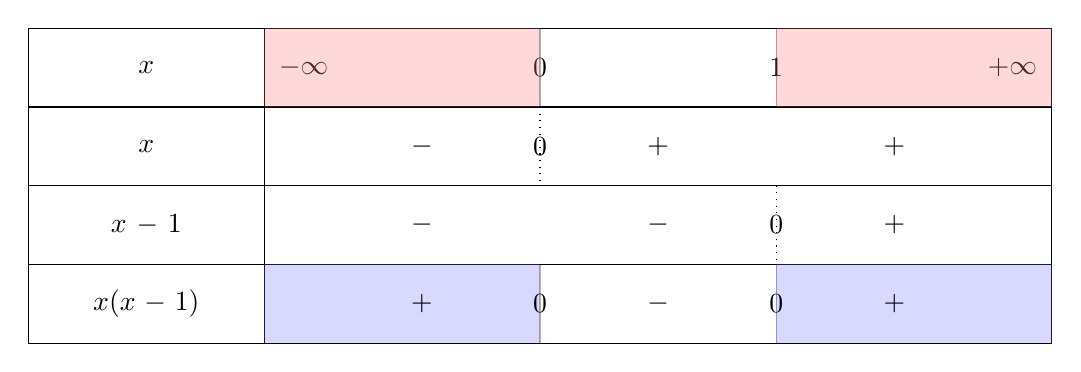
\begin{tikzpicture}[scale=1]
		\tkzTabInit[lgt=3]{$x$ / 1 , $x$ / 1, $x-1$ /1, $x(x-1)$ /1}{$-\infty$, ${\red 0}$ , ${\red 1}$, $+\infty$}
		\draw[fill=red!50, opacity=0.3] (T11) rectangle (N20);
		\draw[fill=red!50, opacity=0.3] (N31) rectangle (T20);
		\draw[fill=blue!50, opacity=0.3] (T14) rectangle (N23);
		\draw[fill=blue!50, opacity=0.3] (N34) rectangle (T23);
		\tkzTabLine{, -, z, +,  , +,  }
		\tkzTabLine{, -,  , -, z, +,  }
		\tkzTabLine{, +, {\blue 0}, -, {\blue 0}, +,  }
\end{tikzpicture}
\end{ExoDec}
}

%%%%%%%%%%%%%%%%%%%%%%%%%%%%%%%%%%%%%%%%%%%%%%%%%%%%%%%%%%%%%%%%%%%
%%%% Page de cours 1
%%%%%%%%%%%%%%%%%%%%%%%%%%%%%%%%%%%%%%%%%%%%%%%%%%%%%%%%%%%%%%%%%%%

\begin{pageCours} % Début page de cours 1

\newgeometry{left=2cm,right=.8cm,top=1.5cm} %Ne pas toucher cette ligne

\section{Première section}

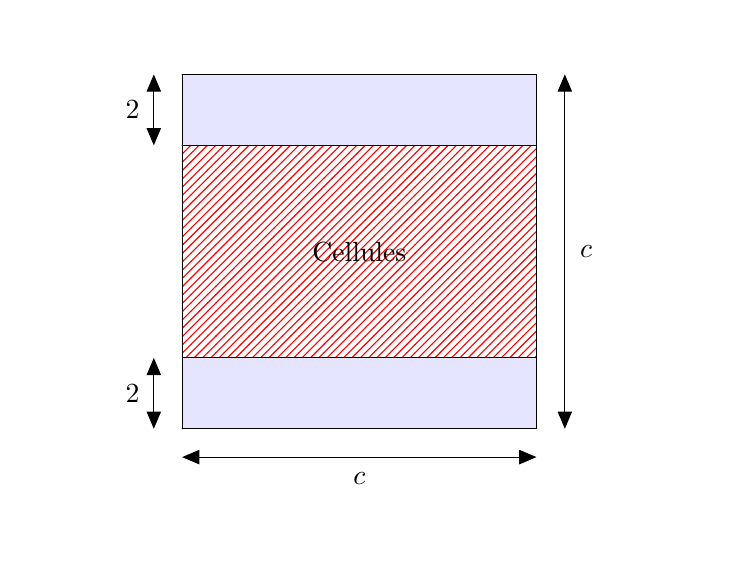
\begin{tikzpicture}[line cap=round,line join=round,>=triangle 45,x=0.9cm,y=0.9cm]
		\clip(-2.18,-1.7) rectangle (7.46,5.66);
\fill[color=blue,fill=blue,fill opacity=0.1] (0,0) -- (5,0) -- (5,1) -- (0,1) -- cycle;
\fill[color=blue,fill=blue,fill opacity=0.1] (0,5) -- (5,5) -- (5,4) -- (0,4) -- cycle;
\fill[pattern color=red,fill=red,pattern=north east lines] (0,4) -- (0,1) -- (5,1) -- (5,4) -- cycle;
\draw (0,0)-- (5,0)-- (5,1)-- (0,1)-- (0,0);
\draw (0,5)-- (5,5)-- (5,4)-- (0,4) -- (0,5);
\draw [<->] (5.4,5)--(5.4,0);
\draw [<->](-0.4,1)--(-0.4,0);
\draw [<->](-0.4,5)--(-0.4,4);
\draw [<->](0,-0.4)--(5,-0.4);
\draw (0,4)--(0,1)--(5,1)--(5,4)--(0,4);
\draw (2.5,2.5) node[anchor=center] {Cellules};
\draw (5.7,2.5) node[anchor=center] {$c$};
\draw (-0.7,4.5) node[anchor=center] {$2$};
\draw (-0.7,0.5) node[anchor=center] {$2$};
\draw (2.5,-0.7) node[anchor=center] {$c$};
\end{tikzpicture}

\begin{tikzpicture}[scale=1,line cap=round,line join=round,>=triangle 45,x=1cm,y=1cm]
	\clip(-0.6,-1.17) rectangle (7.25,3.9);
	\draw plot[samples=100,domain=0:3.141,variable=\t]({3*cos(\t r)+3},{3*sin(\t r)});
	\draw[color=blue, line width=2pt] (4,0)-- (4,2.82842);
	\draw (0,0)-- (4,2.82842);
	\draw (4,2.82842)-- (6,0);
	\draw[color=red, line width=2pt] (3,3)-- (3,0);
	\draw[<->] (0,-0.3)-- (4,-0.3);
	\draw[<->] (4,-0.3)-- (6,-0.3);
	\draw (2.7,1.5) node[anchor=center] {\red $m$};
	\draw (3.6,1.414) node[anchor=north west] {{\blue $g$}};
	\draw (0,0)-- (6,0);
	% les angles droits
	\draw (2.7,0)--(2.7,0.3)--(3,0.3);
	\draw (3.7,0)--(3.7,0.3)--(4,0.3);
	\draw (3.755 , 2.655)--(3.928 , 2.410)--(4.1732,2.583);
	\fill (0,0) circle (1.5pt);
	\draw (-0.2,0) node {$A$};
	\fill  (3,3) circle (1.5pt);
	\draw[color=red] (3.14,3.23) node {$M$};
	\fill (6,0) circle (1.5pt);
	\draw  (6.2,0) node {$B$};
	\fill  (4,0) circle (1.5pt);
	\draw[color=blue] (4.18,0.23) node {$D$};
	\fill [color=xdxdff] (4,2.82842) circle (1.5pt);
	\draw[color=blue] (4.12,3.07) node {$G$};
	\fill [color=qqqqff] (3,0) circle (1.5pt);
	\draw[color=red] (3.2,0.2) node {$O$};
	\draw  (2,-0.5) node[anchor=center] {$a$};
	\draw  (5,-0.5) node[anchor=center] {$b$};
\end{tikzpicture}

{\scriptsize
\begin{tabular}{|c||c|c|c|}
\hline
\parbox[t]{8cm}{L'ensemble des solutions
de $x(x-2)=0$ est} &
$\{2\}$ & $\{0;2\}$ & $\{0;-2\}$ \\\hline
\parbox[t]{8cm}{Soit $a$ un nombre. Le nombre
	de solutions de l'équation $x^2=a$ est}
& $2$ & $1$ & $0$, $1$ ou $2$ \\\hline
\parbox[t]{8cm}{Pour $x \neq 0$, l'équation $\ds\frac{x+2}x=0$
est équivalente à}
& $x+2=0$& $x+2=x$  & $x=2$ \\\hline
\parbox[t]{8cm}{L'équation $x(x+2)=x(2x+3)$ est équivalente
à}
& $x+2=2x+3$& $x=0$ ou $-x-1=0$	 & aucune des 2 autres  \\\hline
\parbox[t]{8cm}{L'équation $(x+2)(x+3)=1$ est équivalente
à}
& $x+2=1$ ou $x+3=1$ & $x+2=1$ et $x+3=1$  & aucune des 2 autres \\\hline
\parbox[t]{8cm}{L'ensemble des solutions
	de $2x-8 \geq 0$ est}
&	$]-\infty;4]$ & $[4;+\infty[$ & $]4;+\infty[$ \\\hline
\parbox[t]{8cm}{L'ensemble des solutions
	de $-5x+8 >3$ est}
&	$]-\infty;-1[$ & $]-\infty;-1]$ & $]11/5;+\infty[$ \\\hline

\parbox[t]{8cm}{
	L'inéquation $\ds\frac{x+2}{-5}>1$
	est équivalente à}
& $x+2>-5$ & $x+2<-5$  & aucune des 2 autres  \\\hline

\parbox[t]{8cm}{L'inéquation $\ds\frac{x+2}x>1$ pour ensemble
	de solutions : }
& $\mathbb R$ & $]-\infty;-2] \cup ]0;+\infty[$  &  $]0;+\infty[$  \\\hline



\parbox[t]{8cm}{Le carré de $x$ est plus grand que $x$ :}
& pour tout $x$ &	pour aucun $x$ & ça dépend de $x$   \\\hline
\end{tabular} 
} 

\begin{DefT}{Titre def}

\end{DefT}

\section{Deuxième section}

\section{Troisième section}

\end{pageCours} % Fin page de cours 1

%%%%%%%%%%%%%%%%%%%%%%%%%%%%%%%%%%%%%%%%%%%%%%%%%%%%%%%%%%%%%%%%%%%
%%%% Application direct 1
%%%%%%%%%%%%%%%%%%%%%%%%%%%%%%%%%%%%%%%%%%%%%%%%%%%%%%%%%%%%%%%%%%%

\begin{pageAD}  % Début page d'exercice d'application direct 1
\restoregeometry %Ne pas toucher cette ligne

\Sf{Premier SF}

\begin{ExoCad}{Compétence.}{1234}{0}{0}{0}{0}{0}

\end{ExoCad}

\Sf{Deuxième SF}

\begin{ExoCad}{Compétence.}{1234}{0}{0}{0}{0}{0}

\end{ExoCad}

\Sf{Troisième SF}

\begin{ExoCad}{Compétence.}{1234}{0}{0}{0}{0}{0}

\end{ExoCad}
 
\end{pageAD} % Fin page d'exercice d'application direct 1

%%%%%%%%%%%%%%%%%%%%%%%%%%%%%%%%%%%%%%%%%%%%%%%%%%%%%%%%%%%%%%%%%%%
%%%% Parcours niveau 1
%%%%%%%%%%%%%%%%%%%%%%%%%%%%%%%%%%%%%%%%%%%%%%%%%%%%%%%%%%%%%%%%%%%

\begin{pageParcoursu} % Début du parcours niveau 1

%Premier exo du parcours 1
\begin{ExoCu}{Compétence.}{1234}{2}{0}{0}{0}{0}
  
\end{ExoCu}

%Deuxième exo du parcours 1
\begin{ExoCuN}{Compétence.}{1}{0}{0}{0}{0}

\end{ExoCuN}

%Troisième exo du parcours 1
\begin{ExoCuN}{Compétence.}{1}{0}{0}{0}{0}

\end{ExoCuN}

%Quatrième exo du parcours 1
\begin{ExoCuN}{Compétence.}{1}{0}{0}{0}{0}

\end{ExoCuN}

%Cinquième exo du parcours 1
\begin{ExoCuN}{Compétence.}{1}{0}{0}{0}{0}

\end{ExoCuN}

%Sixième exo du parcours 1
\begin{ExoCuN}{Compétence.}{1}{0}{0}{0}{0}

\end{ExoCuN}


\end{pageParcoursu} % Fin du parcours niveau 1
 
%%%%%%%%%%%%%%%%%%%%%%%%%%%%%%%%%%%%%%%%%%%%%%%%%%%%%%%%%%%%%%%%%%%
%%%% Parcours Niveau 2
%%%%%%%%%%%%%%%%%%%%%%%%%%%%%%%%%%%%%%%%%%%%%%%%%%%%%%%%%%%%%%%%%%%

\begin{pageParcoursd} % Début du parcours niveau 2

%Premier exo du parcours 2
\begin{ExoCdN}{Compétence.}{2}{0}{0}{0}{0}

\end{ExoCdN}

%Deuxième exo du parcours 2
\begin{ExoCdN}{Compétence.}{2}{0}{0}{0}{0}

\end{ExoCdN}

%Troisième exo du parcours 2
\begin{ExoCdN}{Compétence.}{2}{0}{0}{0}{0}

\end{ExoCdN}

%Quatrième exo du parcours 2
\begin{ExoCdN}{Compétence.}{2}{0}{0}{0}{0}

\end{ExoCdN}

%Cinquième exo du parcours 2
\begin{ExoCdN}{Compétence.}{2}{0}{0}{0}{0}

\end{ExoCdN}

%Sixième exo du parcours 2
\begin{ExoCdN}{Compétence.}{2}{0}{0}{0}{0}

\end{ExoCdN}

\end{pageParcoursd} % Fin du parcours niveau 2

%%%%%%%%%%%%%%%%%%%%%%%%%%%%%%%%%%%%%%%%%%%%%%%%%%%%%%%%%%%%%%%%%%%%
%%%%% Parcours Niveau 3
%%%%%%%%%%%%%%%%%%%%%%%%%%%%%%%%%%%%%%%%%%%%%%%%%%%%%%%%%%%%%%%%%%%%

\begin{pageParcourst} % Début du parcours niveau 3

% Premier exo du parcours 3
\begin{ExoCtN}{Compétence.}{1}{1}{0}{0}{0}
 
\end{ExoCtN}

% Deuxième exo du parcours 3
\begin{ExoCtN}{Compétence.}{1}{1}{0}{0}{0}
 
\end{ExoCtN}

% Troisième exo du parcours 3
\begin{ExoCtN}{Compétence.}{1}{1}{0}{0}{0}
 
\end{ExoCtN}

% Quatrième exo du parcours 3
\begin{ExoCtN}{Compétence.}{1}{1}{0}{0}{0}
 
\end{ExoCtN}

% Cinquième exo du parcours 3
\begin{ExoCtN}{Compétence.}{1}{1}{0}{0}{0}
 
\end{ExoCtN}

% Sixième exo du parcours 3
\begin{ExoCtN}{Compétence.}{1}{1}{0}{0}{0}
 
\end{ExoCtN}
 
\end{pageParcourst} % Fin du parcours niveau 3

%%%%%%%%%%%%%%%%%%%%%%%%%%%%%%%%%%%%%%%%%%%%%%%%%%%%%%%%%%%%%%%%%%%
%%%%  Autoevaluation/exos ouverts
%%%%%%%%%%%%%%%%%%%%%%%%%%%%%%%%%%%%%%%%%%%%%%%%%%%%%%%%%%%%%%%%%%%

\begin{pageAuto} % Début de la page d'exos ouverts

%Premier exercice : "ce que je peux avoir en éval"
\begin{ExoAutoN}{Compétence.}{1}{0}{0}{0}{0}

\end{ExoAutoN}

%Deuxième exercice : "ce que je peux avoir en éval"
\begin{ExoAutoN}{Compétence.}{1}{0}{0}{0}{0}

\end{ExoAutoN}

%%%%%%%%%%%%%%%%%%%%%%%%%%%%%%%%%%%%%%%%%%%%%%%%%%%%%%%%%%%%%%%%%%%
%%%%%%%%%%%%%%%%%%%%%%%%%%%%%%%%%%%%%%%%%%%%%%%%%%%%%%%%%%%%%%%%%%%

%Problème ouvert
\begin{ExoAutoN}{Compétence.}{1}{0}{0}{0}{0}

\end{ExoAutoN}

\end{pageAuto} % Fin de la page d'exos ouverts

%%%%%%%%%%%%%%%%%%%%%%%%%%%%%%%%%%%%%%%%%%%%%%%%%%%%%%%%%%%%%%%%%%%
%%% Page algorithmique
%%%%%%%%%%%%%%%%%%%%%%%%%%%%%%%%%%%%%%%%%%%%%%%%%%%%%%%%%%%%%%%%%%%

\begin{pageAlgo} % Début de la page d'exos d'algorithmique

%Exercice d'algorithmique
\begin{ExoAlgoN}{Compétence.}{1}{0}{0}{0}{0}

\end{ExoAlgoN}

%Exercice d'algorithmique
\begin{ExoAlgo}{Compétence.}{1}{0}{0}{0}{0}

\end{ExoAlgo}

\end{pageAlgo} % Fin de la page d'exos d'algorithmique

%%%%%%%%%%%%%%%%%%%%%%%%%%%%%%%%%%%%%%%%%%%%%%%%%%%%%%%%%%%%%%%%%%%
%%%%  Page(s) blanche(s)
%%%%%%%%%%%%%%%%%%%%%%%%%%%%%%%%%%%%%%%%%%%%%%%%%%%%%%%%%%%%%%%%%%%

\begin{pageBrouillon}

\end{pageBrouillon}

\end{document}
